% ****** Start of file apssamp.tex ******
%
%   This file is part of the APS files in the REVTeX 4.2 distribution.
%   Version 4.2a of REVTeX, December 2014
%
%   Copyright (c) 2014 The American Physical Society.
%
%   See the REVTeX 4 README file for restrictions and more information.
%
% TeX'ing this file requires that you have AMS-LaTeX 2.0 installed
% as well as the rest of the prerequisites for REVTeX 4.2
%
% See the REVTeX 4 README file
% It also requires running BibTeX. The commands are as follows:
%
%  1)  latex apssamp.tex
%  2)  bibtex apssamp
%  3)  latex apssamp.tex
%  4)  latex apssamp.tex
%
\documentclass[superscriptaddress,unsortedaddress,
%runinaddress,
%frontmatterverbose, 
%preprint,
%preprintnumbers,
%nofootinbib,
%nobibnotes,
%bibnotes,
 amsmath,amssymb,
 aps,
%pra,
%prb,
%rmp,
%prstab,
%prstper,
%floatfix,
]{revtex4-2}

\usepackage{graphicx}% Include figure files
\usepackage{dcolumn}% Align table columns on decimal point
\usepackage{bm}% bold math
\usepackage{physics}
\usepackage{lipsum}
\usepackage{subfig}
% \usepackage{braket}
\usepackage{siunitx}
\usepackage{color}
\sisetup{separate-uncertainty}

%\newcommand\abs[1]{\left|#1\right|}
%\newcommand\bra[1]{\left| #1 \right \rangle}
%\newcommand\ket[1]{\left \langle #1 \right |}

\newcommand{\oliver}[1]{\textcolor{violet}{#1}} 
\newcommand{\morten}[1]{\textcolor{green}{#1}}
\newcommand{\sebastian}[1]{\textcolor{cyan}{#1}}
\newcommand{\marianne}[1]{\textcolor{blue}{#1}}
\newcommand{\oyvind}[1]{\textcolor{maroon}{#1}}
\newcommand{\lasse}[1]{\textcolor{red}{#1}}

\begin{document}


\title{Predicting Solid State Qubit Candidates}

\author{Oliver Lerstøl Hebnes}
\affiliation{Department of Physics and Center for Computing in Science Education, University of Oslo, N-0316 Oslo, Norway}

\author{Marianne Etzelm\"uller Bathen}
\affiliation{Advanced Power Semiconductor Laboratory, ETH Zürich, 8092  Zürich,  Switzerland}
\affiliation{Department of Physics and Center for Materials Science and Nanotechnology, University of Oslo, N-0316 Oslo, Norway}

\author{Øyvind Sigmundson Schøyen}
\affiliation{Department of Physics and Center for Computing in Science Education, University of Oslo, N-0316 Oslo, Norway}

\author{Sebastian G. Winther-Larsen}
\affiliation{Department of Physics and Center for Computing in Science Education, University of Oslo, N-0316 Oslo, Norway}

\author{Morten Hjorth-Jensen}
\affiliation{Facility for Rare Ion Beams and Department of Physics and Astronomy, Michigan State University, East Lansing, MI 48824, USA}
\affiliation{Department of Physics and Center for Computing in Science Education, University of Oslo, N-0316 Oslo, Norway}

\author{Lasse Vines}
\affiliation{Department of Physics and Center for Materials Science and Nanotechnology, University of Oslo, N-0316 Oslo, Norway}

\begin{abstract}

Semiconductor materials provide a compelling platform for quantum
technology, and a vast amount of materials and their properties can be
found in high-throughput databases.  However, filtering among these
materials in order to find novel candidates for quantum technology is
a challenge. Therefore, we provide a framework for the automatic
discovery of promising solid-state material hosts using machine
learning methods.

%Main message 1: develop methodology for data mining and machine learning for materials properties 
We have developed data extraction tools for numerous material science
databases, and constructed over $4800$ physics-informed features for a
dataset consisting of more than $25000$ materials.  Furthermore, we
have developed and implemented three data mining approaches, termed
\textit{the Ferrenti approach}, \textit{the augmented Ferrenti
  approach} and \textit{the insightful approach} for defining three
distinct training sets for the supervised machine learning algorithms
logistic regression, decision tree, random forest and gradient boost
to be trained on.

% Main message 2: Use method to propose new materials that are promising quantum hosts 
We find a lack of consistent results for the Ferrenti approach and the
augmented Ferrenti approach due to an overly broad formulation of the
training set, whereas the restrictions set in the insightful approach
proved suitable. All models agreed on $214$ predicted candidates, with
examples such as ZnGeP$_2$, MgSe, CdS, BP, BC$_2$N, BP, Ge, GeC, InP,
and InAs. All approaches and all models agreed on a subset of $47$
eligible candidates of $8$ elemental, $29$ binary, and $10$ tertiary
compounds.

\end{abstract}

\pacs{02.70.Ss, 31.15.A-, 31.15.bw, 71.15.-m, 73.21.La}




\maketitle

%Submit to npj Computational Materials

%Marianne: I have now structured the paper according to other papers in this journal 
%I think we can make a supplementary material if we see that we need it, it is quite common for the journal 

\section*{Introduction}%Oliver and Morten and Marianne (semiconductor portion)
The second quantum revolution is heralding the development of new solutions and devices based on quantum technology \cite{Acin2018}. Among the promising prototypes that are already available we find in vivo sensing of magnetic fields in cells [], secure communication over large distances by separation of entangled photons, and finally the demonstration of quantum computers []. 
Quantum computers in particular are in high demand to sate the continued demand for computing power strong enough to solve increasingly complex problems. 
Recently, the potential of such machines to outperform classical systems was proven when a 53-qubit quantum computer based on superconductor electronics solved a computational problem that was beyond the capabilities of a 200'000 core supercomputer \cite{Arute_2019}, spurring further investigations into competitive quantum technology platforms.  

Quantum platforms are available but both the materials and fabrication technologies are far less mature than those for, e.g., classical computers and sensors. 
An important concern in this context is that of scalability. 
For example, the best performing quantum computer prototypes rely on either superconducting electronics or trapped ions. Both technologies require millikelvin temperatures to operate, fabrication is challenging, and the stability of interactions is an issue. 
Instead, semiconductors are emerging as a promising alternative platform, offering competitive characteristics combined with the possibility of room temperature operation and mature and scalable material processing and fabrication.  

Quantum technologies based on semiconductors rely on either defects or quantum dots, where the latter kind can be of the self-assembled or the fabricated type. 

%From thesis - rewrite 
Unfortunately, there are substantial challenges associated with the modern quantum platforms simultaneously as the selection of quantum platforms are slim. The majority of discoveries of potential quantum platforms have so far happened by serendipity, and there is an urgent need for new and better materials that can escalate the effort for a sustainable future. 

The fourth science paradigm introduces the potential of targeted search for promising material systems to act as qubit hosts. 
Herein, we provide a framework for the automatic discovery of promising solid-state material hosts using machine learning methods. 
Initial database building similar to Ferrenti et al \cite{Ferrenti2020}. 

\begin{figure}[t]
    \centering
    \includegraphics[width=0.9\textwidth]{figures/paradigms.png}
    \caption{[PLACEHOLDER] Schematic over paradigms in science.}
    \label{fig:paradigm}
\end{figure}

\section*{Theoretical Background and Experimental Data} 
%Not all papers have a theory chapter, but since we are speaking to two quite different communities, it might be nice to include some basics. 

%Some of this can also be copied into the introduction 

Quantum technologies, including sensing, communication and computing, 
are intriguing because of the new capabilities they offer. 
However, realization of large-scale fabrication for these techniques requires further technological development. 
The superconducting electronics platform that is currently employed for quantum computers necessitates millikelvin temperatures and may prove challenging to scale. 
Instead, recent developments have seen/heralded the rise of semiconductors as possible host materials for a variety of quantum devices. Semiconductor quantum dots or point defects could prove easier to combine with existing devices, and room temperature operation of prototype communication and computing devices has been shown.  
However, this technology is still in the early stages, and the issues left to address include scalable and reproducible device fabrication, identification of ideally suited host candidates, and, importantly, understanding the requirements for a material to act as a good host remain unclear. 
%Different methods are needed. 

\subsection*{Semiconductors as a Quantum Host} %Marianne and Lasse 
Quantum technologies commonly rely on a quantum bit or qubit as the basis for operation. 
\marianne{Some schematic is shown in Figure~\ref{fig:qt}}. 
For all applications, the basic requirement is a two-level quantum system which is essentially isolated from its environment, ensuring sufficient stability to perform various operation. In other words, we search for systems which exhibit a high degree of coherence. Additionally, the qubit state must be controlable via repeatable initialization, manipulation and read-out protocols.  
A set of requirements were formulated by DiVincenzo for the case of qubits and quantum computing \cite{DiVincenzo2000}. Below, these are rephrased to encompass qubit requirements for all three QT application areas:  
\begin{itemize}
    \item A scalable physical system with well-characterized qubits
    \item Reliable qubit initialization protocols 
    \item Quantum gates and protocols to operate on and control qubit states  
    \item Qubit state coherence time must exceed gate operation time 
    \item Qubit state read-out after operation, preferably optically.  
\end{itemize}

\begin{figure}[t]
    \centering
    \includegraphics[width=0.4\textwidth]{figures/qubit.png}
    \caption{[PLACEHOLDER] Schematic of classical versus quantum bits. }
    \label{fig:qt}
\end{figure}

%Discuss experimental data and the semiconductor platform. 
Semiconductors embody point defects that may trap charge carriers, causing deep energy levels to appear within the fundamental band gap. 
Importantly, deep level defects can trap carriers in localized states that are essentially isolated from the surroundings, making them suitable for QT. 
A prime example is the nitrogen-vacancy (NV) center in diamond, which has been proposed 
as a contender for both computing, sensing and communication applications \cite{Doherty_2013}. 
The NV center is a room temperature single-photon source emitting in the visible portion of the spectrum, and has been employed for, e.g., stress tensor mapping \cite{Broadway2019} and optical imaging of living cells \cite{Lesage_2013}.  
Moreover, the NV center in its negative charge state traps an electron in a localized and high-spin $S=1$ state that can be coherently controlled and with RT spin coherence times above \SI{1}{\milli\second} \cite{Doherty_2013}, 
leading to demonstrations of entanglement and teleportation of two NV center spins \cite{Bernien2013,Pfaff_2014}. 
However, despite these promising discoveries, diamond  as a quantum platform comes with several important drawbacks. The relevant defects therein, such as the NV center, emit in the visible region of the spectrum which is not compatible with the telecom wavelengths needed to integrate with optical fiber technology. 
Additionally, diamond is expensive, device fabrication is challenging and scalability is poor, leading to concerns in whether quantum technology device development will be realizable on this platform. 
Hence, we search among the plethora of available semiconductors for a platform that can deliver on the necessary parameters for QT applications while also, ideally, providing availability and scalable fabrication. 
In this context, the material properties that facilitate quantum compatible characteristics such as single-photon emission and coherent spin manipulation to manifest must be identified. 

\begin{table}[h]
    \centering
    \caption{Overview of materials and defects that have been demonstrated to exhibit QT compatible characteristics such as single-photon emission and coherent spin manipulation.}
    \begin{tabular}{c|c|c|c}
    Material & Band gap (eV) & Defect candidates & References \\
    \hline
    Diamond  & $5.5$  & N$_\mathrm{C}V_\mathrm{C}$, Si$_\mathrm{C}V_\mathrm{C}$, Ge$_\mathrm{C}V_\mathrm{C}$ & \cite{Balasubramanian_2009,Rogers_2014,Bhaskar_2018} \\ 4H-SiC & $3.3$ & $V_\mathrm{Si}$, $V_\mathrm{Si}V_\mathrm{C}$, C$_\mathrm{Si}V_\mathrm{C}$, N$_\mathrm{C}V_\mathrm{Si}$ & \cite{Widmann2014,Christle_2015,Castelletto_2014,Zargaleh_2018} \\ 
    Si & $1.1$ & P, G, unidentified & \cite{Muhonen_2014,Durand_2020,Redjem2020} \\ 
    (2D) \textit{h}-BN & $6.0$ & Unidentified defects & \cite{Tran_2016,Tran_2016b,Hayee_2020} \\ 
    ZnO & $3.4$ & Unidentified defects & \cite{Morfa2012} \\ 
    ZnS & $3.6$ (zincblende) & Unidentified defects & \cite{Stewart2019} \\ 
    GaAs & $1.4$ & Quantum dots & \cite{Bluhm2010} \\ 
    GaN & $3.4$ & Quantum dots, unidentified defects & \cite{Roux2017,Berhane2018} \\
    AlN & $6.0$ & Unidentified defects & \cite{Xue2020}\\
    \end{tabular}
    \label{tab:qt-materials}
\end{table}

%\begin{figure}[t]
%    \centering
%    \includegraphics[width=0.5\textwidth]{figures/NV.png}
%    \caption{[PLACEHOLDER] Schematic representation of the electronic structure of the NV center in diamond.}
%    \label{fig:defects-dft}
%\end{figure}

\begin{figure}[t]
    \centering
    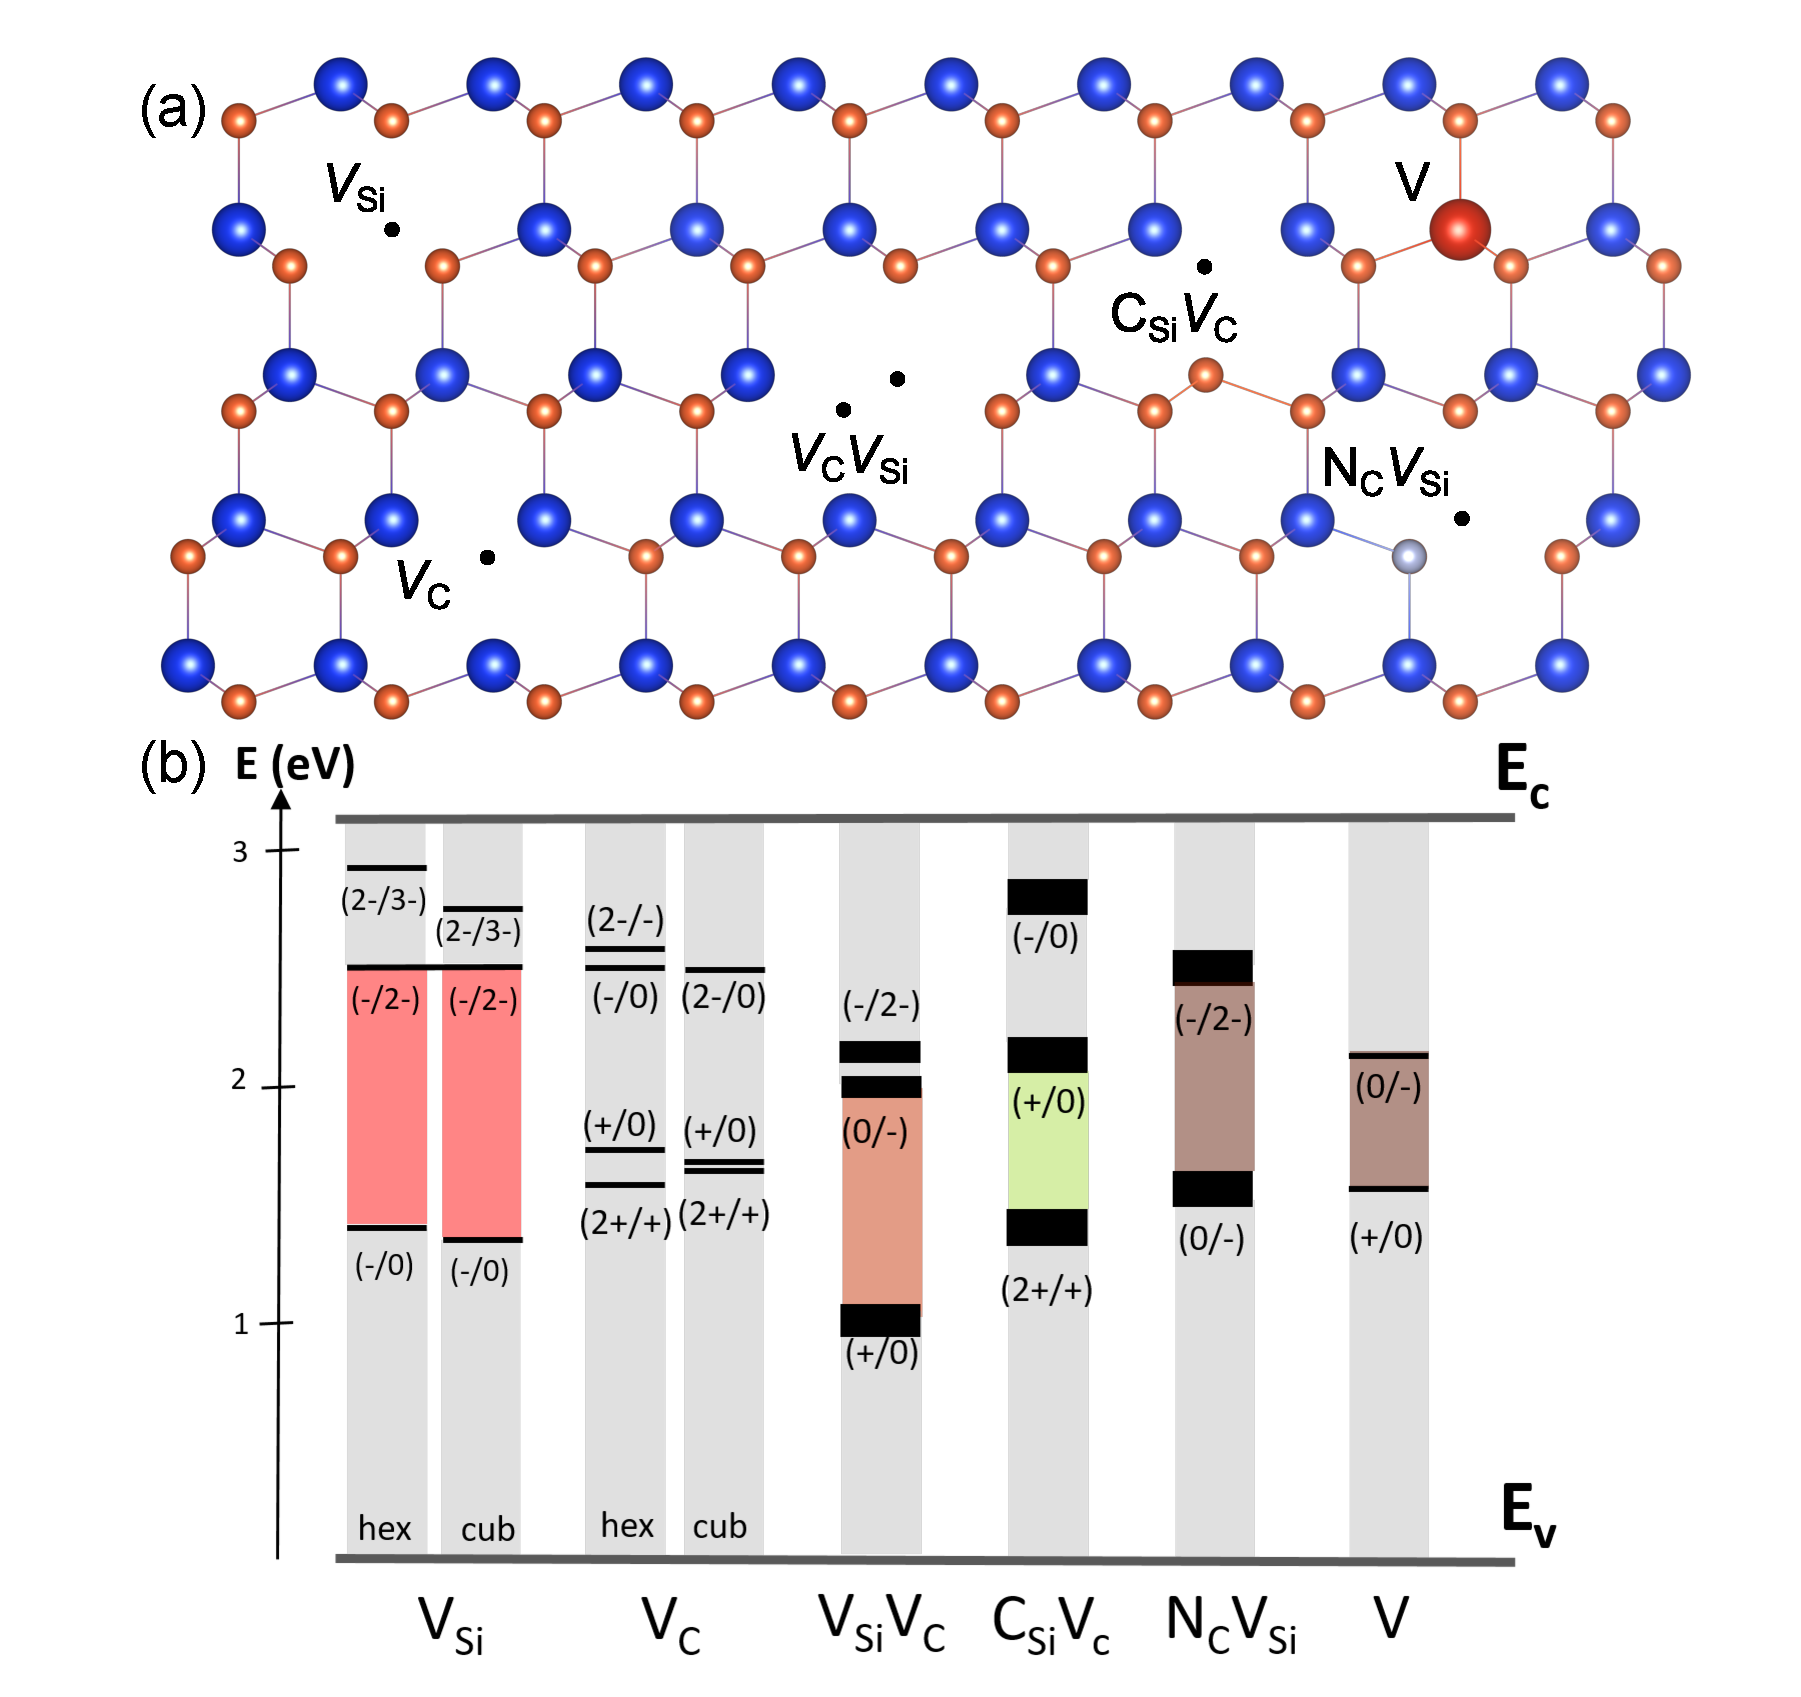
\includegraphics[width=0.5\textwidth]{figures/defects-sic.pdf}
    \caption{[PLACEHOLDER] Schematic representation of different quantum compatible defects in SiC and the energy levels they introduce into the band gap, from Ref.\cite{Bathen2021}.} 
    \label{fig:defects-sic}
\end{figure}

%QT requirements. 
%What parameters are we looking for? 
Table \ref{tab:qt-materials} contains an overview of known semiconductor materials with demonstrated quantum compatible characteristics. In this context we consider single-photon emission and coherent spin manipulation for systems related to point defects primarily, but also self-assembled or lithographically structured quantum dots. 
\marianne{A (placeholder) schematic of quantum compatible defects and the energy levels they introduce into the band gap of 4H-SiC is shown in Figure~\ref{fig:defects-sic}.}
Most of the defects in the table have yet to be identified, and different material related challenges complicate the implementation of defects for QT. 
A set of common denominators for materials that contain qubit defects was summarized by Weber et al. \cite{Weber2010}: 
\begin{itemize}
    \item Wide band gap to facilitate localized deep levels (physical)
    \item Low spin orbit coupling to extend spin coherence times (physical) 
    \item Low el-phonon coupling for sharp emission lines (physical) 
    \item Availability as high-quality, bulk, or thin-film single crystals (practical)
    \item Constituent elements with naturally occurring isotopes of zero nuclear spin (practical). 
\end{itemize}
Note the division between physical and practical requirements in the list above. 
The physical criteria refer to some fundamental aspect of the material that permits specific properties to manifest, while practical refers to the external influences that simplify measurement and detection of the interesting properties. 
In this work, we will focus primarily on the former set of criteria, as understanding them better may give further insights into the makings of a reliable QT platform. 

In addition to obtaining greater understanding of  exactly what constitutes a good quantum host material, we must recognize that different defect and material types may suit different needs. Therefore, we aim to develop a bigger bank of candidate defects and materials. 
So far, detection of QT compatibility in semiconductors has been rather slow, depending on signal detection and later identification in each specific material. 
Instead, we are looking for a top-down approach to \textit{predict} promising materials, enabling a guiding of experimental efforts. 
%For this, we first need a large dataset. 

\subsection*{Density Functional Theory Output} %Marianne 
The density functional theory (DFT) is a versatile and powerful theoretical approach that has been exceptionally successful in predicting solid-state material properties such as stability of different phases, lattice parameters and band gaps. 
DFT provides a method for iteratively solving the Schr{\"o}dinger equation based on initial guesses for the atomic potentials. 
Using DFT calculations, we are able to accurately investigate semiconductor materials with many atoms while keeping efficiency and cost in mind.  

%DFT is based on the Hohenberg-Kohn \cite{Hohenberg1964} and Kohn-Sham \cite{Kohn1965} theorems and provides a method for iteratively solving the Schrodinger equation based on initial guesses for the atomic potentials. 
%The foundation for DFT centers around the electronic density providing all ground-state properties of the system, provided that the external potential can be exactly described. 
%The fundamental challenge of DFT calculations is that this potential, as expressed by the exchange-correlation functional, can be exactly computed for only very few and simple systems.

The fundamental challenge of the DFT is that the calculations rely on approximations to the potential function of a system as expressed by the exchange-correlation (XC) functional, which is not known for bulk materials. 
The XC functional is usually grouped into three categories based on the level of theory. The local density approximation (LDA) takes the homogeneous electron gas as a starting point, while the more advanced general gradient approximation (GGA) includes also the gradient in local electron gas variations. 
These local or semi-local functionals yield satisfactory results on geometrical concerns but tend to underestimate energies such as the band gap or defect energy levels due to a self-interaction error (i.e., an electron is allowed to interact with itself) [Ref SchollSteckel] \cite{Freysoldt2014}. 
More recent developments have seen the widespread use of hybrid functionals such as the HSE06 incorporating a portion of Hartree-Fock exact exchange \cite{Heyd2003},  albeit at a much greater computational cost. 
%See, e.g., this review \cite{Freysoldt2014} for further details on different functionals for semiconductor and defect calculations. 

Despite the limitations imposed by the approximate nature of the XC functional, and the band gap error of LDA and GGA level functionals, 
DFT can be a powerful tool when predicting, designing and interpreting experiments. 
Herein, we employ databases containing DFT calculations of material properties to gain insight into the fundamental mechanisms behind observed quantum characteristics, and predict new candidate QT hosts. 
The calculations we employ were performed using the GGA-level Perdew-Burke-Erznerhof (PBE) functional \cite{Perdew1996}. 
Note that the PBE functional tends to underestimate the band gap of semiconductor materials.  
Nonetheless, a larger data set is available than for, e.g., HSE06, and many trends are conserved also with PBE. 
The ground-state (and $0$~K) parameters that can be extracted from this type of data set include the total energy (translates into stability), the band gap, the electronegativity, the electron-phonon coupling and magnetic properties. 

\subsection*{Material Informatics} %Øyvind (Oliver)    
%Data mining, screening 

\begin{figure}[t]
    \centering
    \includegraphics[width=\textwidth]{figures/ht-workflow.jpg}
    \caption{[PLACEHOLDER for workflow] Morten: can you please add the other schematic figure we discussed as placeholder? Sebastian makes our own versions of these schematic figures (I can make some VESTA files with materials). }
    \label{fig:ht-workflow}
\end{figure}

\subsection*{Machine Learning} % Morten 

\section*{Results}
Includes discussion of results.  

\subsection*{Information Flow}  %Sebastian/Oyvind (Marianne) 
% MEB: Since Methods are at the end, I propose to put part of this
% discussion in the Results section. 
% This is because it is an important result of the work, and also
% because it is important to understand the rest of the paper 

The information stream of this project can be regarded as many
modular parts connected in logical pieces. The initial step for
gathering and building features is visualized by the
the flowchart in [INSERT FIGURE!!]. 
Initially, we start by extracting all entries in
the Materials Project that matches a specific query. 
Thereafter, we apply Matminer’s\cite{Ward2018}
featurization tools to make thousands
of features of the data. The conditions on this initial query are that the
materials must
derive from experimental data, and have a band gap wider than $0.1$ eV.
In a parallel step, entries that are deemed
similar to the entries from the initial query
are extracted from AFLOW\cite{Curtarolo2012, Curtarolo2012a, Calderon2015},
AFLOW-ML\cite{Isayev2017},
JARVIS-DFT, % \cite{Choudhary2020},
OQMD\cite{Saal2013,Kirklin2015}
and
Citrine Informatics. The results of these steps are combined into
a data set for further analysis.


% \subsection*{Optimization of Machine Learning Models} %Morten (Oliver input in round 2)

\subsection*{Data Mining}

After compiling a dataset from the procedure outlined above, we 
face a challenge in terms of defining a training set that we can 
train data on. This is not only challenging due to the lack of known
suitable candidates (1), but also due to the intricacy of defining
materials as unsuitable candidates (0). We follow three separate
procedures to this end.

\subsubsection*{The Ferrenti approach}

The first approach to defining a training set is based on the criteria
from the paper by \citeauthor{Ferrenti2020} \cite{Ferrenti2020}.
They suggest a data mining process consisting of four stages by 
systematically evaluating the suitability of host materials from
the Materials Project.

We label \textbf{suitable} candidates by the following steps.

\begin{enumerate}
    \item Include materials that;
    \begin{itemize}
        \item contain elements with more than $50\%$ natural abundance of 
            zero spin isotopes,
        \item crystallize in nonpolar space groups,
        \item is present in the ICSD database, and
        \item is calculated nonmagnetic
    \end{itemize}
    \item Pragmatically remove toxic, radioactive and otherwise 
        ``difficult'' materials;
    \begin{itemize}
        \item exclude Th, U, Cd and Hg,
        \item exclude any rare-earth metals and noble gases,
        \item exclude Ru, Os, Fe or Ni.
    \end{itemize}
    \item Include only materials with a band gap larger than $0.5$eV by MP
        PBE-GGA.
    \item Ensure energy above hull is less than $0.2$ eV per atom.
\end{enumerate}

We then label \textbf{un}-suitable candidates amongst materials in 
the ICSD database that crystallize in polar space groups, are calculated
to be magnetic and have a band gap larger than $0.1$ eV by MP PBE-GGA.

\subsubsection*{The augmented Ferrenti approach}
In the second approach, we adjust the first approach in order to
improve the dataset. This approach is therefore named
\emph{the augmented Ferrenti Approach}.

In the first approach we included critera that were not motivated by physically 
motivated, but from a purely practical perspective, like excluding toxic and
radioactive elements. Such criteria is not necessarily related to what makes 
a material suitable for quantum technology - eventually it is up to the 
experimentalist to decide the practicability of the employed material.
Consequently, we remove stage two from the approach above. What is more, we will
include a few more elements that has shown promising properties (REF??), but were
initially excluded due to the lack of spin-zero isotopes. 

The following steps make up the process of choosing \textbf{suitable} candidates 
in the \emph{augmented Ferrenti approach},
\begin{enumerate}
    \item Include materials that,
    \begin{itemize}
        \item contain elements where more than half have a natural abundance of zero spin
            isotopes, except Al, P, Ga, As, B and N.
        \item crystallize in non-polar space groups,
        \item is present in the ICSD database,
        \item is calculated nonmagnetic.
    \end{itemize}
    \item Only keep materials that have a band gap larger than 1.5 eV as
        calculated by MP PBE-GGA,
    \item Ensure energy above hull is less than 0.2 eV per atom. 
\end{enumerate}

For \textbf{unsuitable} candidates, we implement the same strategy as the non-augmented
Ferrenti approach. The result is a somewhat unbalanced dataset, with up to 75 \% of the 
materials found in the suitable group. However, the dataset is 78 \% larger than in
approach 1.

\subsubsection*{The insightful approach}
The third approach is vastly different from the two first approaches in terms
of labeling, as we apply knowledge from the field (REFS!!) 
to pick our promising material host candidates. We therefore name this scheme 
\emph{the insightful approach}.
Due to the concern of having a too-small dataset, we will include
materials that are promising and have shown suitable properties to
accommodate deep defects that potentially can exhibit quantum effects.
The approach to pick \textbf{suitable} candidates can be summed up as,
\begin{enumerate}
    \item Pick candidates that match the formulas [A BUNCH OF MATERIALS AND REFERENCES HERE] and are present in the ICSD database.  
    \item Perform a manual screening for correct structures.
\end{enumerate}

After the first stage of picking candidates we are left with a list of 202 matching formulas which include 12 entries that have a band gap of less than $0.4$~eV. These structures are unstable in terms of energy above hull calculations, and will decompose other materials in the list with a band gap that is substantially above 0.5 eV. We include all except C (mp-568410),
with MP-computed band gap of 0.12 eV - a metal according to AFLOW-ML and therefore 
labeled as unsuitable instead.

MORE ON MANUAL SCREENING....

Since the dataset constituting suitable candidates are few, we add 400 \emph{unsuitable}
candidates. These are picked at random from the pool of unsuitable candidates 
from the two previous approaches, in addition to those that are marked unsuitable through
the manual screening process.

\subsubsection*{Comparing the approaches}

Figure 5.3 would be nice to have here :) Also figure 5.4.


\subsection*{Predicting Novel Material Hosts for Quantum Technology} %Sebastian / Oyvind (Oliver input in round 2) 

\section*{Discussion} % All - last thing we write  
Shorter section, includes summary, concluding remarks and is quite heavy on outlook.  

\section*{Methods}
Should be rather short. Details can be included in a Supplementary Material. 

\subsection*{Information Flow}

\subsection*{Databases} %Sebastian, Oliver and Øyvind 
The Materials Project (REF) is an open-source project based on the Vienna Ab Initio Package (VASP) (REF). The functional GGA is used to calculate band structures, while for transition metals, a $+U$ correction is applied to correct for correlation effects (REF). The project is known as the initiator of materials genomics and offers a variety of calculated properties of over one hundred thousand inorganic crystalline materials, with frequent updates and extensions. 

The AFLOW (REF) repository is an automatic software framework that utilize the GGA-PBE functional within VASP. 



%Materials project, AFLOW, Open Quantum, JARVIS 
Mining.  

\subsection*{Material Informatics} %Oliver and Øyvind 
Screening and workflow and approaches.  

\subsection*{Machine Learning} %Sebastian/Morten   
Insight gaining. 

\section*{Data availability} 
%We can put something else, standard text 
The data that support the plots within this paper and other findings of this study are
available from the corresponding authors upon reasonable request. [Marianne: I assume you want to add the Github link here?] 

\section*{Code availability} 
The codes developed in this study are available from the authors upon reasonable
request. [Marianne: I assume you want to add the Github link here?] 

\bibliography{apssamp}% Produces the bibliography via BibTeX.

\begin{acknowledgments}

The work of MHJ is supported by the U.S. Department of Energy,
Office of Science, office of Nuclear Physics under grant
No. DE-SC0021152 and U.S. National Science Foundation Grants
No. PHY-1404159 and PHY-2013047. 
The work of MEB and LV was supported by the Research Council of Norway and the University of Oslo through the frontier research project FUNDAMeNT (no. 251131, FriPro ToppForsk-program). 
%Some of the computations were performed on resources provided by UNINETT Sigma2 - the National Infrastructure for High Performance Computing and Data Storage in Norway.  
The work of MEB was supported by an ETH Zurich Postdoctoral Fellowship. 

\end{acknowledgments}

\section*{Author contributions} 
%Copied in from another paper 
S.-M.J. conceived the idea and developed the simulation model. T.H.L. performed
computer simulation. S.Y.B. and S.D.H. fabricated devices. D.-W.S., S.L., H.W.C. and
J.-W.J. supported measurement of device performances. Y.-H.S. and X.-B.F.
synthesised QD materials. S.Z. and J.Y. supported experiments. C.S. and Y.K.
supported computer simulation. L.G.O. and G.A. supported data analysis. J.M.K.
guided this work. S.-M.J., T.H.L. and S.Y.B. contributed equally. 
All the authors contributed to the preparation of the manuscript.

\section*{Competing interests}
The authors declare no competing interests.


\end{document}

